\chapter{Specifikacija programske potpore}
		
	\section{Funkcionalni zahtjevi}
			
			\textbf{\textit{dio 1. revizije}}\\
			
			\textit{Navesti \textbf{dionike} koji imaju \textbf{interes u ovom sustavu} ili  \textbf{su nositelji odgovornosti}. To su prije svega korisnici, ali i administratori sustava, naručitelji, razvojni tim.}\\
				
			\textit{Navesti \textbf{aktore} koji izravno \textbf{koriste} ili \textbf{komuniciraju sa sustavom}. Oni mogu imati inicijatorsku ulogu, tj. započinju određene procese u sustavu ili samo sudioničku ulogu, tj. obavljaju određeni posao. Za svakog aktora navesti funkcionalne zahtjeve koji se na njega odnose.}\\
			
			
			\noindent \textbf{Dionici:}
			
			\begin{packed_enum}
				
				\item Zaposlenik
				\item Revizor
				\item Računovođa
				\item Direktor
				\item Razvojni tim
				
			\end{packed_enum}
			

			\noindent \textbf{Aktori i njihovi funkcionalni zahtjevi:}
			
			\begin{packed_enum}
				\item  \underbar{Svaki neregistrirani/neprijavljeni korisnik (inicijator) može:}

				\begin{packed_enum}
					
					\item prijaviti se u sustav
					
				\end{packed_enum}
			
				\item  \underbar{Svaki registrirani/prijavljeni korisnik (inicijator) može:}
				
				\begin{packed_enum}
					
					\item promijeniti lozinku korisničkog računa
					\item vidjeti povijest svojih skeniranja dokumenata
					\item skenirati novi dokument i:

						\begin{packed_enum}
							
							\item potvrditi točnost skeniranog dokumenta
							\item odbiti skenirani dokument

						\end{packed_enum}
					
					\item odjaviti se iz sustava

				\end{packed_enum}

				\item  \underbar{Zaposlenik (inicijator) može:}
				
				\begin{packed_enum}
					
					\item poslati skenirani dokument revizoru na reviziju
					
				\end{packed_enum}

				\item  \underbar{Revizor (inicijator) može:}
				
				\begin{packed_enum}
					
					\item provjeriti pristigle dokumente, uključujući svoje, i:

						\begin{packed_enum}
							
							\item potvrditi dokument i proslijediti ga nadležnom računovođi
							\item odbiti dokument

						\end{packed_enum}
					
				\end{packed_enum}

				\item  \underbar{Računovođa (inicijator) može:}

				\begin{packed_enum}
					
					\item arhivirati pristigle dokumente
					\item proslijediti pristigli dokument direktoru na potpis
					
				\end{packed_enum}

				\item  \underbar{Direktor (inicijator) može:}

				\begin{packed_enum}
					
					\item potpisati dokumente pristigle iz računovodstva
					\item vidjeti povijest svih skeniranja dokumenata
					\item vidjeti povijest skeniranja i statistike svih zaposlenika
					\item objaviti određeni dokument na društvenim mrežama 
					\item registrirati novog korisnika i dodijeliti mu ulogu
					\item obrisati postojećeg korisnika
					
				\end{packed_enum}

				\item  \underbar{Baza podataka (sudionik):}

				\begin{packed_enum}

					\item pohranjuje sve podatke o korisnicima i njihovim ovlastima (ulogama)
					\item pohranjuje sve podatke o skeniranim dokumentima
					
				\end{packed_enum}			

			\end{packed_enum}
	
			\eject{}
			
			\subsection{Obrasci uporabe}
				
				\subsubsection{}

					\noindent \underbar{\textbf{UC1 — Prijava u sustav}}
					\begin{packed_item}
	
						\item \textbf{Glavni sudionik:} Bilo koji korisnik
						\item  \textbf{Cilj:} Dobiti pristup korisničkom sučelju
						\item  \textbf{Sudionici:} Baza podataka
						\item  \textbf{Preduvjet:} Posjedovanje vlastitog korisničkog računa
						\item  \textbf{Opis osnovnog tijeka:}
						
						\item[] \begin{packed_enum}
	
							\item Korisnik unosi korisničko ime i lozinku
							\item Baza podataka provjerava ispravnost unesenih podataka
							\item Korisnik dobiva pristup korisničkom sučelju

						\end{packed_enum}
						
						\item  \textbf{Opis mogućih odstupanja:}
						
						\item[] \begin{packed_item}
	
							\item[2.a] Korisnik je unio neispravno korisničko ime ili lozinku
							\item[] \begin{packed_enum}
								
								\item Sustav obavještava korisnika o neuspjeloj prijavi i vraća ga na stranicu za prijavu
								
							\end{packed_enum}
							
						\end{packed_item}

					\end{packed_item}


					\noindent \underbar{\textbf{UC2 — Promjena lozinke korisničkog računa}}
					\begin{packed_item}
	
						\item \textbf{Glavni sudionik:} Bilo koji korisnik
						\item  \textbf{Cilj:} Promijeniti lozinku korisničkog računa
						\item  \textbf{Sudionici:} Baza podataka
						\item  \textbf{Preduvjet:} Korisnik je prijavljen u sustav
						\item  \textbf{Opis osnovnog tijeka:}
						
						\item[] \begin{packed_enum}
	
							\item Korisnik odabire opciju promjene lozinke računa
							\item Korisnik unosi trenutnu lozinku računa
							\item Baza podataka provjerava ispravnost unesene lozinke
							\item Korisnik unosi novu lozinku računa
							\item Baza podataka pohranjuje promjenu lozinke

						\end{packed_enum}
						
						\item  \textbf{Opis mogućih odstupanja:}
						
						\item[] \begin{packed_item}
	
							\item[3.a] Korisnik je unio neispravnu trenutnu	lozinku
							\item[] \begin{packed_enum}
								
								\item Sustav obavještava korisnika o pogrešnom unosu trenutne lozinke i vraća ga na stranicu za unos lozinke
								
							\end{packed_enum}
							
						\end{packed_item}

					\end{packed_item}


					\noindent \underbar{\textbf{UC3 — Pregled povijesti skeniranih dokumenata}}
					\begin{packed_item}
	
						\item \textbf{Glavni sudionik:} Zaposlenik
						\item  \textbf{Cilj:} Vidjeti povijest svojih skeniranja dokumenata
						\item  \textbf{Sudionici:} Baza podataka
						\item  \textbf{Preduvjet:} Korisnik je prijavljen u sustav
						\item  \textbf{Opis osnovnog tijeka:}
						
						\item[] \begin{packed_enum}
	
							\item Aplikacija korisniku na početnom zaslonu prikazuje njegovu povijest skeniranih dokumenata

						\end{packed_enum}

					\end{packed_item}


					\noindent \underbar{\textbf{UC4 — Skeniranje novog dokumenta}}
					\begin{packed_item}
	
						\item \textbf{Glavni sudionik:} Bilo koji korisnik
						\item  \textbf{Cilj:} Skenirati novi dokument
						\item  \textbf{Sudionici:} Baza podataka
						\item  \textbf{Preduvjet:} Korisnik je prijavljen u sustav
						\item  \textbf{Opis osnovnog tijeka:}
						
						\item[] \begin{packed_enum}
	
							\item Korisnik na početnom zaslonu odabire opciju za skeniranje novog dokumenta
							\item Korisnik učitava jedan ili više dokumenata u slikovnom formatu u aplikaciju
							\item Aplikacija provjerava ispravnost učitanih dokumenata
							\item Aplikacija korisniku prikazuje učitani dokument i razvsrtava ga u jednu od kategorija:

								\begin{packed_enum}
									
									\item račun
									\item ponuda
									\item interni dokument

								\end{packed_enum}

							\item Korisnik potvrđuje točnost učitanog dokumenta ili ga odbija

						\end{packed_enum}

						\item  \textbf{Opis mogućih odstupanja:}
						
						\item[] \begin{packed_item}
	
							\item[3.a] Dokument nije ispravno skeniran
							\item[] \begin{packed_enum}
								
								\item Aplikacija obavještava korisnika o neuspjelom skeniranju te uzroku pogreške i vraća ga na zaslon za učitavanje dokumenta
								
							\end{packed_enum}
							
						\end{packed_item}

					\end{packed_item}


					\noindent \underbar{\textbf{UC5 — Slanje skeniranog dokumenta na reviziju}}
					\begin{packed_item}
	
						\item \textbf{Glavni sudionik:} Zaposlenik
						\item  \textbf{Cilj:} Poslati skenirani dokument revizoru na reviziju
						\item  \textbf{Sudionici:} Baza podataka, revizor
						\item  \textbf{Preduvjet:} Zaposlenik je prijavljen u sustav i skenirao je dokument
						\item  \textbf{Opis osnovnog tijeka:}
						
						\item[] \begin{packed_enum}
	
							\item Zaposlenik odabire opciju za slanje skeniranog dokumenta na reviziju
							\item Aplikacija od baze podataka traži popis svih revizora
							\item Baza podataka vraća aplikaciji popis svih revizora
							\item Aplikacija zaposleniku prikazuje popis svih revizora
							\item Zaposlenik odabire revizora kojemu želi poslati dokument
							\item Aplikacija šalje dokument odabranom revizoru te o tome obavještava bazu podataka

						\end{packed_enum}

					\end{packed_item}


					\noindent \underbar{\textbf{UC6 — Provjera pristiglih dokumenata}}
					\begin{packed_item}
	
						\item \textbf{Glavni sudionik:} Revizor
						\item  \textbf{Cilj:} Provjeriti pristigle dokumente, uključujući svoje
						\item  \textbf{Sudionici:} Baza podataka, zaposlenik, računovođa
						\item  \textbf{Preduvjet:} Revizor je prijavljen u sustav i ima pristiglih dokumenata
						\item  \textbf{Opis osnovnog tijeka:}
						
						\item[] \begin{packed_enum}
	
							\item Revizor odabire opciju za provjeru pristiglog dokumenta
							\item Aplikacija revizoru prikazuje dokument
							\item Revizor potvrđuje točnost dokumenta ili ga odbija:
							
							\begin{packed_enum}
								
								\item točan dokument aplikacija prosljeđuje nadležnom računovođi te o tome obavještava bazu podataka
								\item netočan dokument aplikacija odbacuje i o tome dojavljuje zaposlenika

							\end{packed_enum}

						\end{packed_enum}

					\end{packed_item}


					\noindent \underbar{\textbf{UC7 — Arhiviranje pristiglih dokumenata}}
					\begin{packed_item}
	
						\item \textbf{Glavni sudionik:} Računovođa
						\item  \textbf{Cilj:} Arhivirati pristigle dokumente
						\item  \textbf{Sudionici:} Baza podataka
						\item  \textbf{Preduvjet:} Računovođa je prijavljen u sustav i ima pristiglih dokumenata
						\item  \textbf{Opis osnovnog tijeka:}
						
						\item[] \begin{packed_enum}
	
							\item Računovođa odabire opciju za arhiviranje pristiglog dokumenta
							\item Aplikacija dojavljuje bazi podataka da arhivira dokument
							\item Baza podataka arhivira dokument i dodjeljuje mu jedinstveni broj arhiva

						\end{packed_enum}

					\end{packed_item}


					\noindent \underbar{\textbf{UC8 — Slanje dokumenata na potpis direktoru}}
					\begin{packed_item}
	
						\item \textbf{Glavni sudionik:} Računovođa
						\item  \textbf{Cilj:} Poslati dokument direktoru na potpis
						\item  \textbf{Sudionici:} Baza podataka, direktor
						\item  \textbf{Preduvjet:} Računovođa je prijavljen u sustav i ima pristiglih dokumenata
						\item  \textbf{Opis osnovnog tijeka:}
						
						\item[] \begin{packed_enum}
	
							\item Računovođa odabire opciju za slanje dokumenta direktoru na potpis
							\item Aplikacija šalje dokument direktoru na potpis te o tome obavještava bazu podataka
							\item Direktor dobiva obavijest o pristiglom dokumentu

						\end{packed_enum}

					\end{packed_item}


					\noindent \underbar{\textbf{UC9 — Potpisivanje dokumenata}}
					\begin{packed_item}
	
						\item \textbf{Glavni sudionik:} Direktor
						\item  \textbf{Cilj:} Potpisati dokumente pristigle iz računovodstva
						\item  \textbf{Sudionici:} Baza podataka, računovođa
						\item  \textbf{Preduvjet:} Direktor je prijavljen u sustav i ima pristiglih dokumenata
						\item  \textbf{Opis osnovnog tijeka:}
						
						\item[] \begin{packed_enum}
	
							\item Direktor odabire opciju za potpisivanje dokumenta
							\item Aplikacija dojavljuje bazi podataka da je dokument potpisan
							\item Baza podataka označava dokument kao potpisan
							\item Aplikacija šalje potpisani dokument računovođi

						\end{packed_enum}

					\end{packed_item}


					\noindent \underbar{\textbf{UC10 — Pregled povijesti dokumenata}}	
					\begin{packed_item}
	
						\item \textbf{Glavni sudionik:} Direktor
						\item  \textbf{Cilj:} Vidjeti povijest svih dokumenata
						\item  \textbf{Sudionici:} Baza podataka
						\item  \textbf{Preduvjet:} Direktor je prijavljen u sustav
						\item  \textbf{Opis osnovnog tijeka:}
						
						\item[] \begin{packed_enum}
	
							\item Aplikacija direktoru na početnom zaslonu prikazuje povijest svih skeniranja dokumenata

						\end{packed_enum}

					\end{packed_item}


					\noindent \underbar{\textbf{UC11 — Pregled povijesti i statistika zaposlenika}}
					\begin{packed_item}
	
						\item \textbf{Glavni sudionik:} Direktor
						\item  \textbf{Cilj:} Vidjeti povijest i statistike svih zaposlenika
						\item  \textbf{Sudionici:} Baza podataka
						\item  \textbf{Preduvjet:} Direktor je prijavljen u sustav
						\item  \textbf{Opis osnovnog tijeka:}
						
						\item[] \begin{packed_enum}
	
							\item Aplikacija direktoru na početnom zaslonu prikazuje povijest i statistike svih zaposlenika

						\end{packed_enum}

					\end{packed_item}


					\noindent \underbar{\textbf{UC12 — Registracija novog korisnika}}
					\begin{packed_item}
	
						\item \textbf{Glavni sudionik:} Direktor
						\item  \textbf{Cilj:} Registrirati novog korisnika i dodijeliti mu ulogu
						\item  \textbf{Sudionici:} Baza podataka
						\item  \textbf{Preduvjet:} Direktor je prijavljen u sustav
						\item  \textbf{Opis osnovnog tijeka:}
						
						\item[] \begin{packed_enum}
	
							\item Direktor odabire opciju za registraciju novog korisnika
							\item Aplikacija prikazuje formu za registraciju novog korisnika
							\item Direktor unosi podatke o novom korisniku, uključujući njegovu ulogu
							\item Aplikacija provjerava ispravnost unesenih podataka
							\item Aplikacija dojavljuje bazi podataka da registrira novog korisnika
							\item Baza podataka pohranjuje podatke o novom korisniku

						\end{packed_enum}

						\item  \textbf{Opis mogućih odstupanja:}
						
						\item[] \begin{packed_item}
	
							\item[4.a] Direktor je unio neispravne podatke o novom korisniku
							\item[] \begin{packed_enum}
								
								\item Aplikacija obavještava direktora o neuspjeloj registraciji i vraća ga na formu za registraciju novog korisnika

							\end{packed_enum}
							
						\end{packed_item}

					\end{packed_item}


					\noindent \underbar{\textbf{UC13 — Brisanje postojećeg korisnika}}
					\begin{packed_item}
	
						\item \textbf{Glavni sudionik:} Direktor
						\item  \textbf{Cilj:} Obrisati postojećeg korisnika
						\item  \textbf{Sudionici:} Baza podataka
						\item  \textbf{Preduvjet:} Direktor je prijavljen u sustav i postojeći korisnik registriran je u sustavu
						\item  \textbf{Opis osnovnog tijeka:}
						
						\item[] \begin{packed_enum}
	
							\item Direktor odabire opciju za brisanje postojećeg korisnika
							\item Aplikacija prikazuje popis svih korisnika
							\item Direktor odabire korisnika kojeg želi obrisati
							\item Aplikacija dojavljuje bazi podataka da obriše korisnika
							\item Baza podataka briše korisnika

						\end{packed_enum}

					\end{packed_item}


					\noindent \underbar{\textbf{UC14 — Objavljivanje dokumenta na društvene mreže}}
					\begin{packed_item}
	
						\item \textbf{Glavni sudionik:} Direktor
						\item  \textbf{Cilj:} Objaviti određeni dokument na društvene mreže
						\item  \textbf{Sudionici:} Baza podataka, društvene mreže
						\item  \textbf{Preduvjet:} Direktor je prijavljen u sustav i dokument je potpisan
						\item  \textbf{Opis osnovnog tijeka:}
						
						\item[] \begin{packed_enum}
	
							\item Direktor odabire opciju za objavljivanje dokumenta na društvene mreže
							\item Aplikacija direktoru prikazuje izbor društvenih mreža
							\item Direktor odabire društvenu mrežu na koju želi objaviti dokument
							\item Aplikacija direktora preusmjerava na odabranu društvenu mrežu

						\end{packed_enum}

					\end{packed_item}


					\noindent \underbar{\textbf{UC15 — Odjava iz sustava}}
					\begin{packed_item}
	
						\item \textbf{Glavni sudionik:} Korisnik
						\item  \textbf{Cilj:} Odjaviti se iz sustava
						\item  \textbf{Sudionici:} —
						\item  \textbf{Preduvjet:} Korisnik je prijavljen u sustav
						\item  \textbf{Opis osnovnog tijeka:}
						
						\item[] \begin{packed_enum}
	
							\item Korisnik odabire opciju za odjavu iz sustava
							\item Aplikacija korisnika odjavljuje iz sustava i preusmjerava na stranicu za prijavu

						\end{packed_enum}

					\end{packed_item}

				\eject{}
					
				\subsubsection{Dijagrami obrazaca uporabe}

					\begin{figure}[H]
						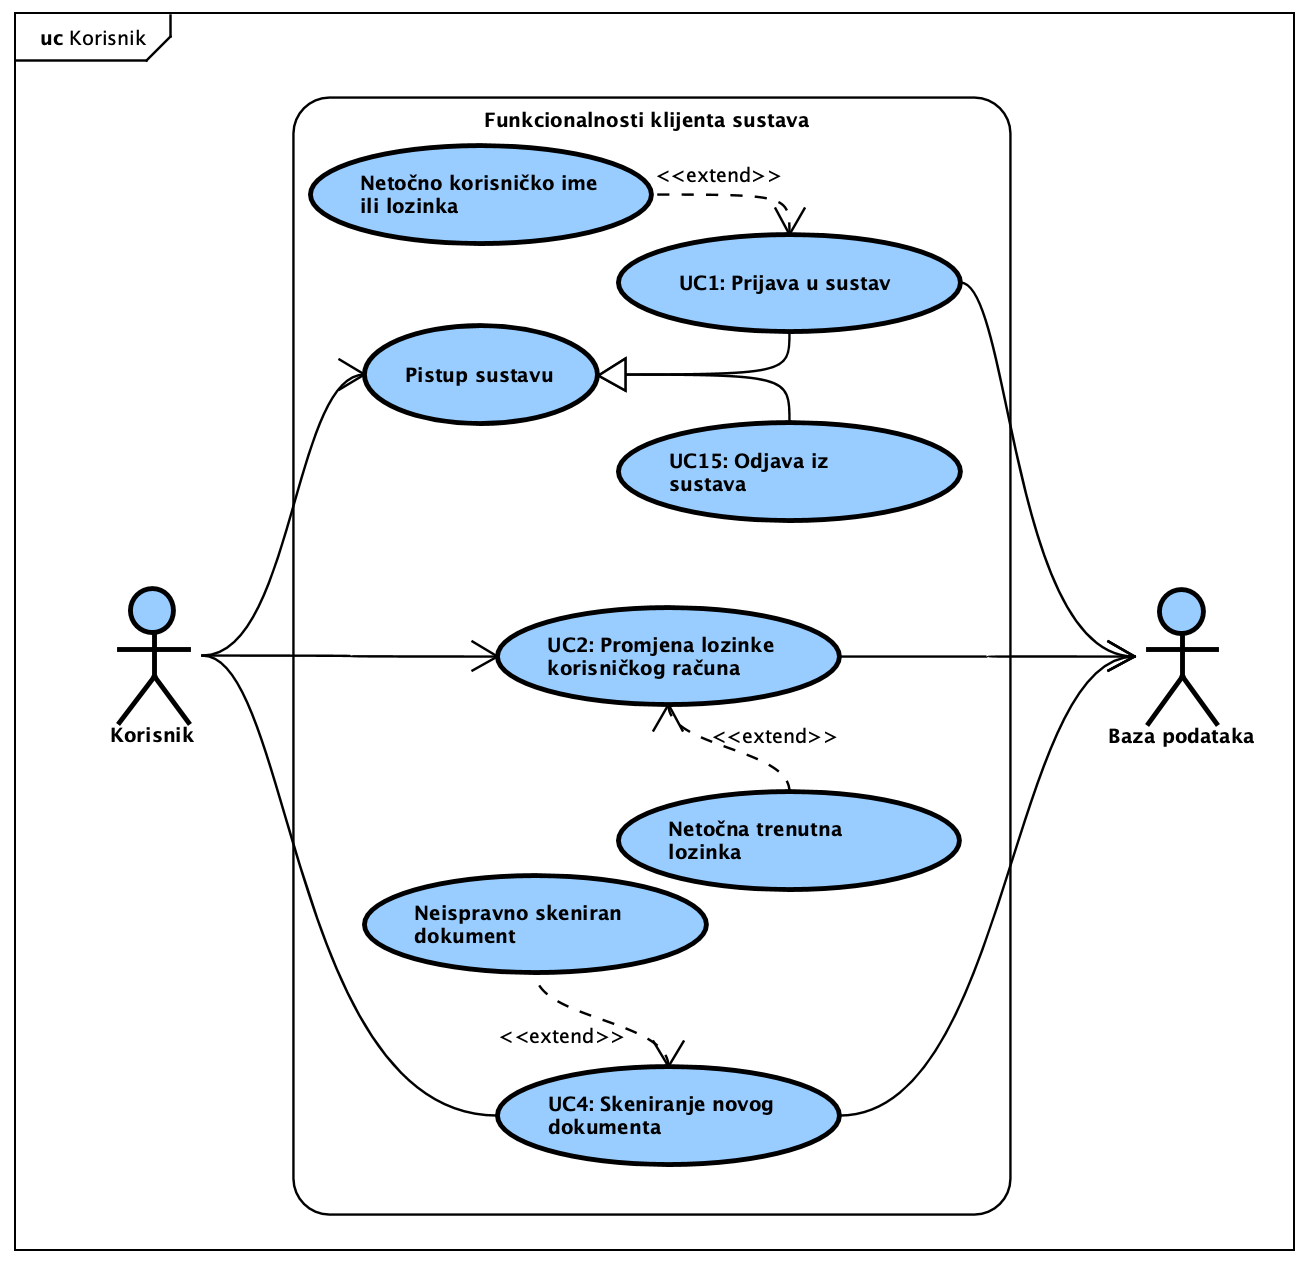
\includegraphics[width=\textwidth]{slike/UseCase_Korisnik.png} %veličina u odnosu na širinu linije
						\caption{Dijagram obrasca uporabe, funkcionalnost korisnika}
						\label{fig:usecase_korisnik} %label mora biti drugaciji za svaku sliku
					\end{figure}

					\begin{figure}[H]
						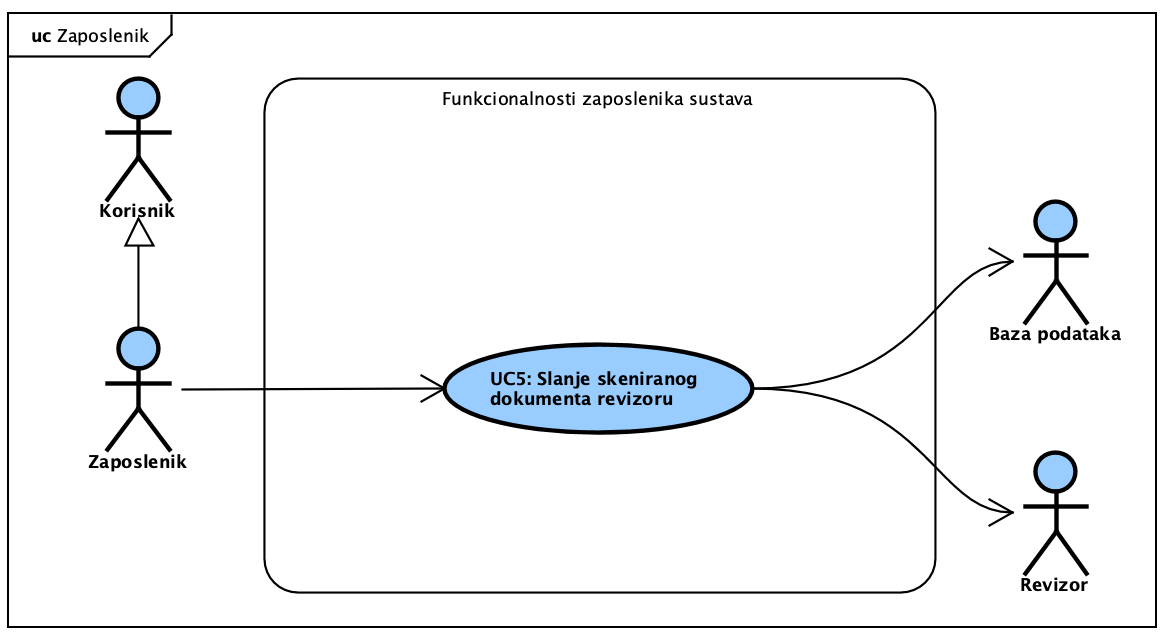
\includegraphics[width=\textwidth]{slike/UseCase_Zaposlenik.png}
						\caption{Dijagram obrasca uporabe, funkcionalnost zaposlenika}
						\label{fig:usecase_zaposlenik}
					\end{figure}

					\begin{figure}[H]
						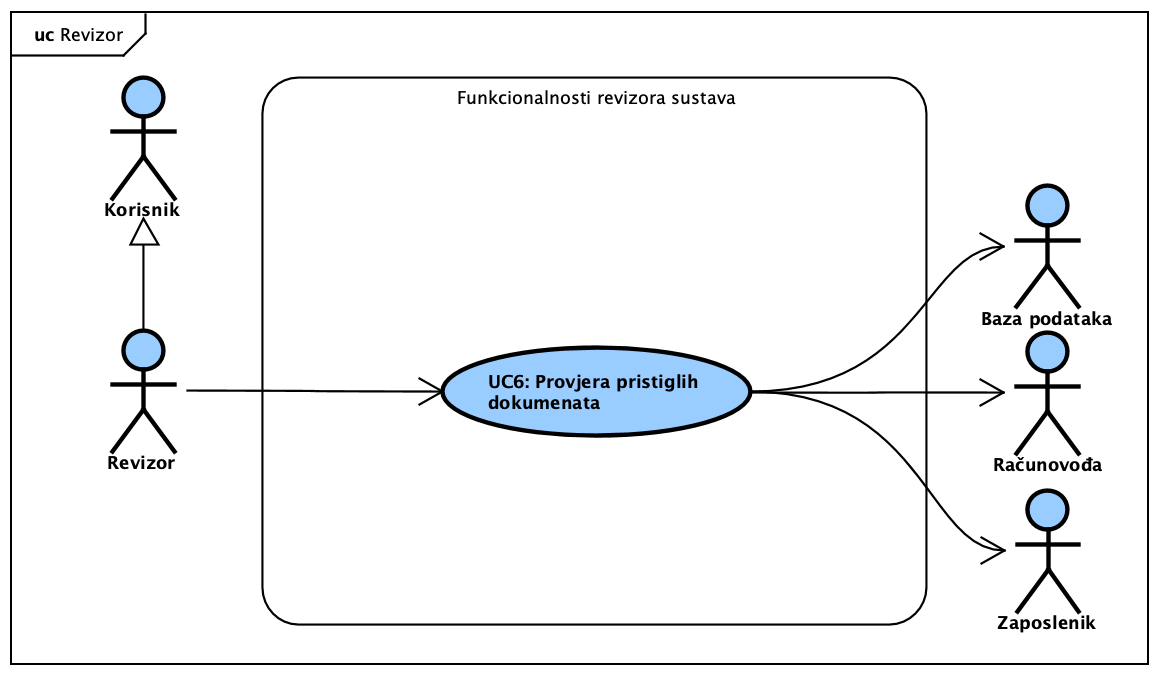
\includegraphics[width=\textwidth]{slike/UseCase_Revizor.png}
						\caption{Dijagram obrasca uporabe, funkcionalnost revizora}
						\label{fig:usecase_revizor}
					\end{figure}

					\begin{figure}[H]
						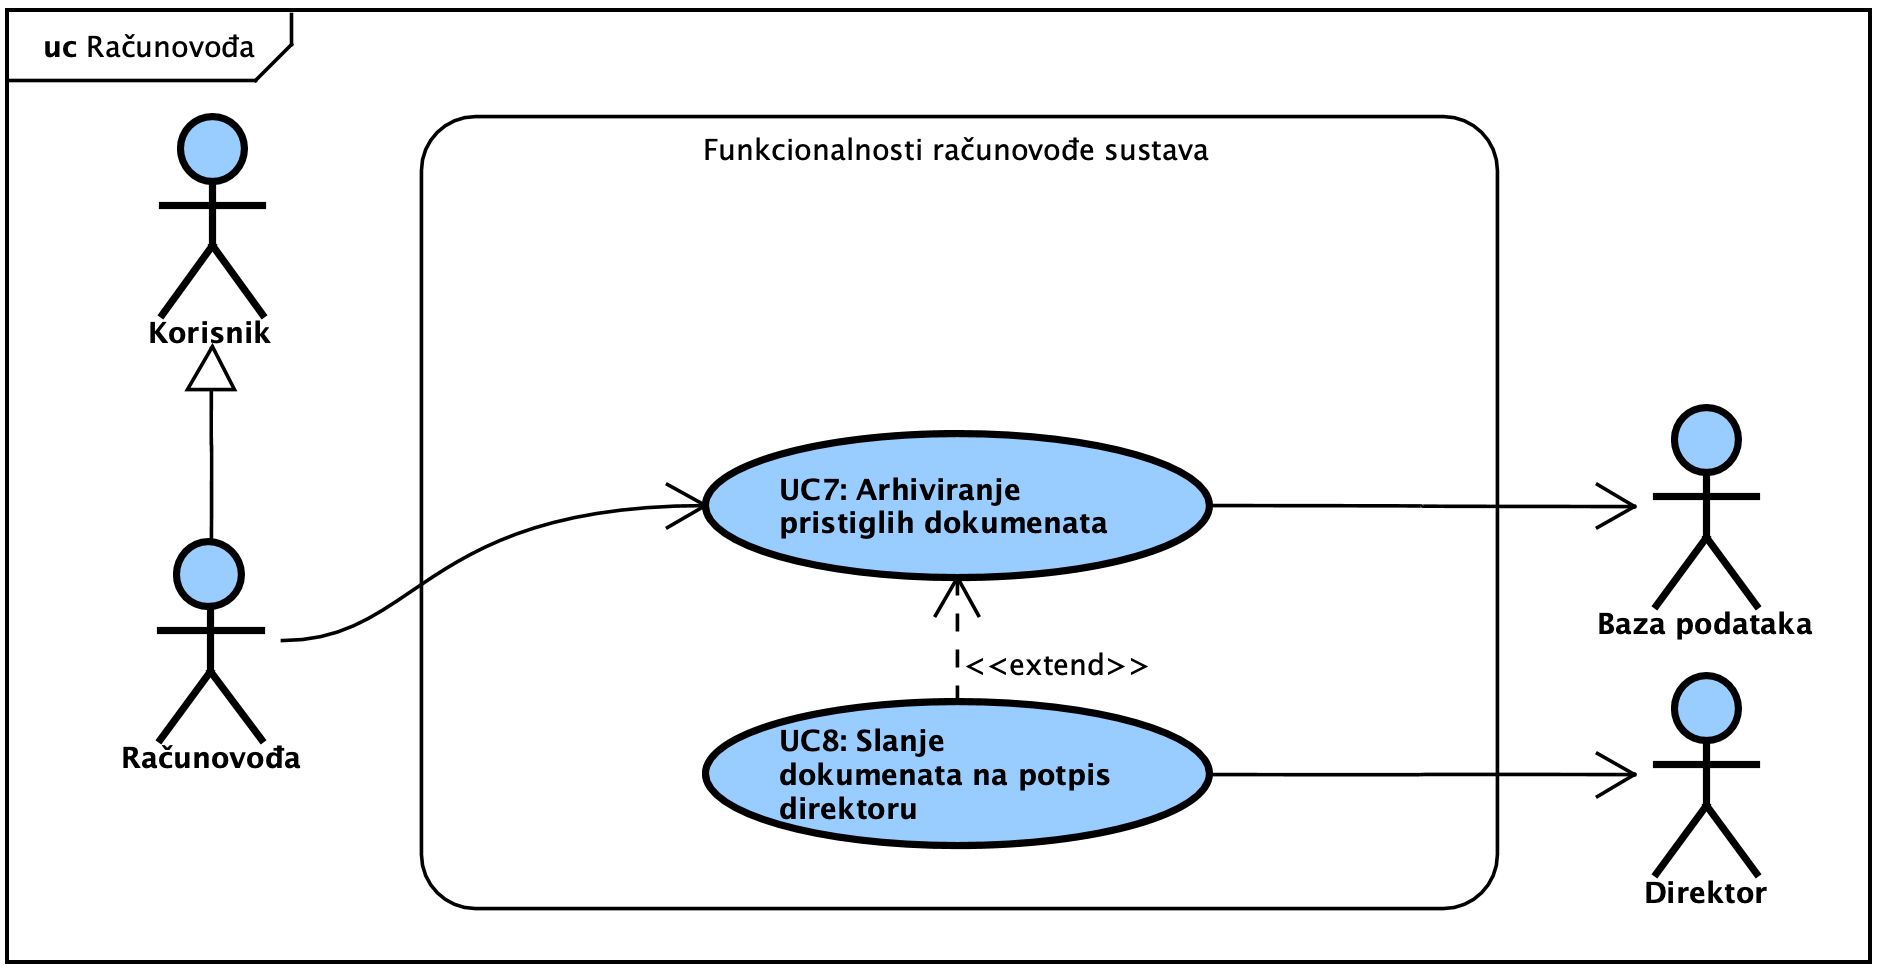
\includegraphics[width=\textwidth]{slike/UseCase_Racunovoda.png}
						\caption{Dijagram obrasca uporabe, funkcionalnost računovođe}
						\label{fig:usecase_racunovoda}
					\end{figure}

					\begin{figure}[H]
						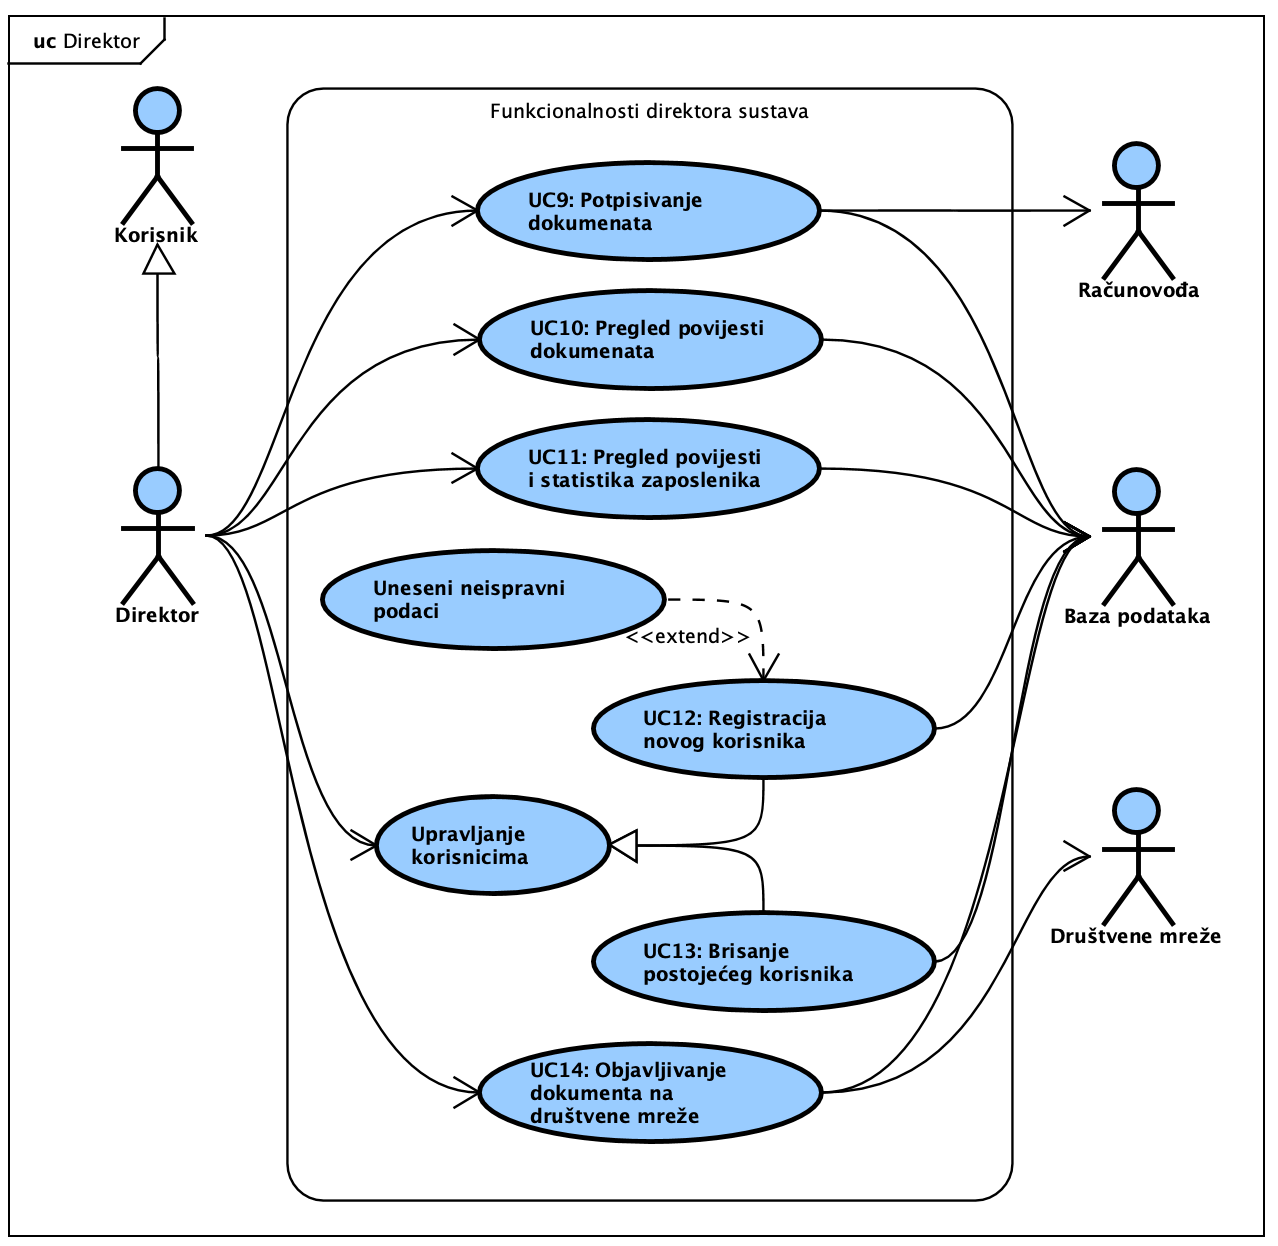
\includegraphics[width=\textwidth]{slike/UseCase_Direktor.png}
						\caption{Dijagram obrasca uporabe, funkcionalnost direktora}
						\label{fig:usecase_direktor}
					\end{figure}
				\eject{}
				
			\subsection{Sekvencijski dijagrami}
				
				\textbf{\textit{dio 1. revizije}}\\

				\begin{figure}[H]
					\textbf{Obrazac uporabe UC1 - Prijava u sustav}
					\text{Korisnik na stranici za prijavu u sustav unosi korisničko ime i lozinku. Aplikacija bazi podataka šalje unesene podatke, baza provjerava njihovu ispravnost te vraća podatke o korisniku. Ukoliko je korisnik unio neispravno
					korisničko ime ili lozinku, baza to javlja aplikaciji koja obavještava korisnika o neuspjeloj prijavi i vraća ga na stranicu za prijavu. Ako su uneseni podaci ispravni sustav korisniku daje pristup korisničkom sučelju.}
					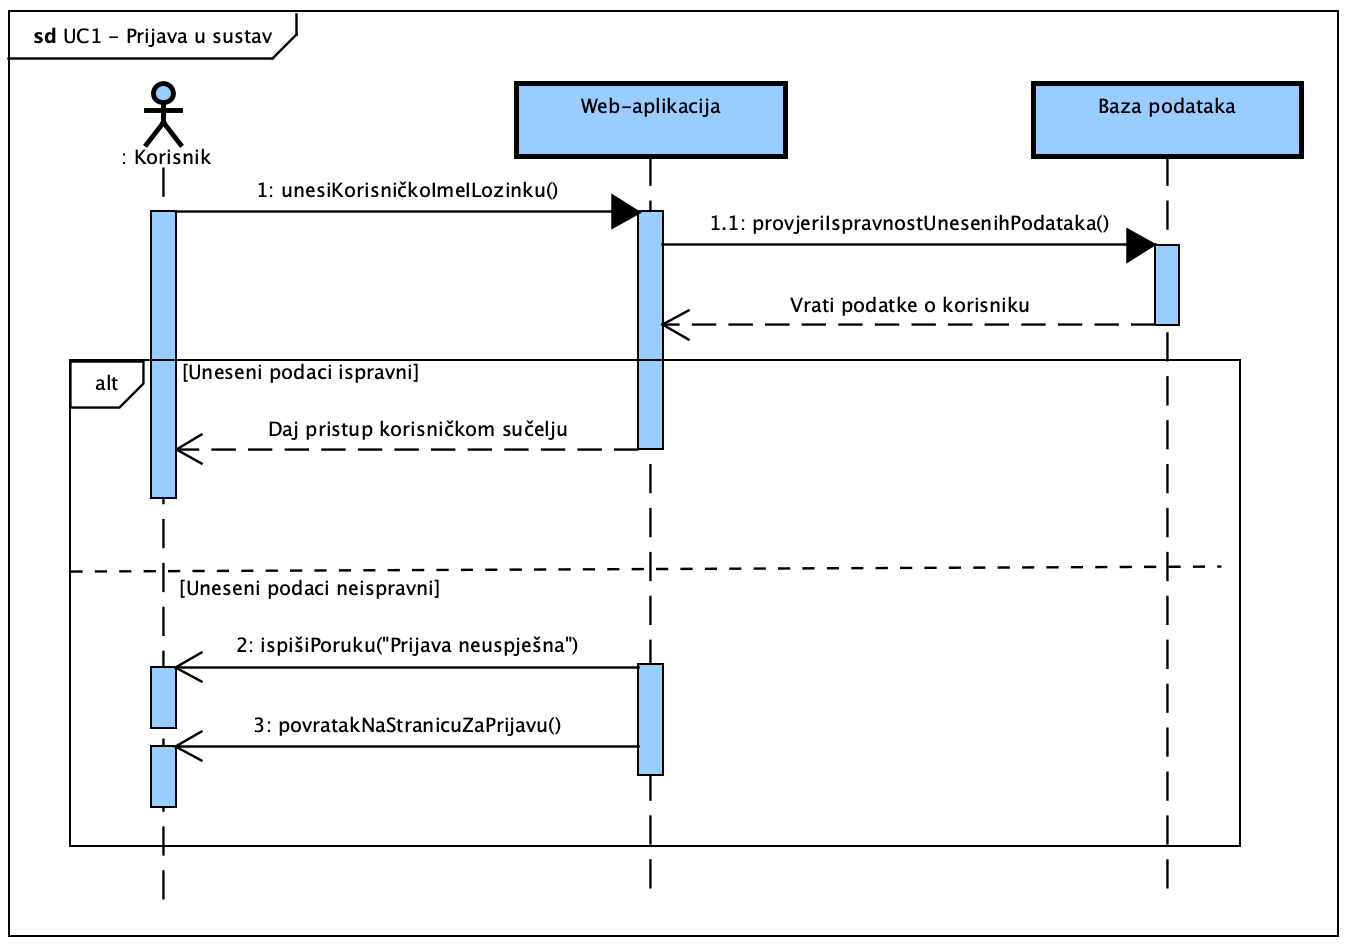
\includegraphics[width=\textwidth]{slike/Sequence_UC01.png}
					\caption{Sekvencijski dijagram za UC01}
					\label{fig:sequence_UC01}
				\end{figure}

				\begin{figure}[H]
					\textbf{Obrazac uporabe UC7 - Arhiviranje pristiglih dokumenata}
					\text{Računovođa aplikaciji šalje zahtjev za prikaz opcija te dabire opciju za arhiviranje pristiglog dokumenta. Aplikacija dojavljuje bazi podataka da arhivira dokument.
					Baza podataka arhivira dokument i dodjeljuje mu jedinstveni broj arhiva te ga vraća aplikaciji, koja ga prikazuje računovođi.}
					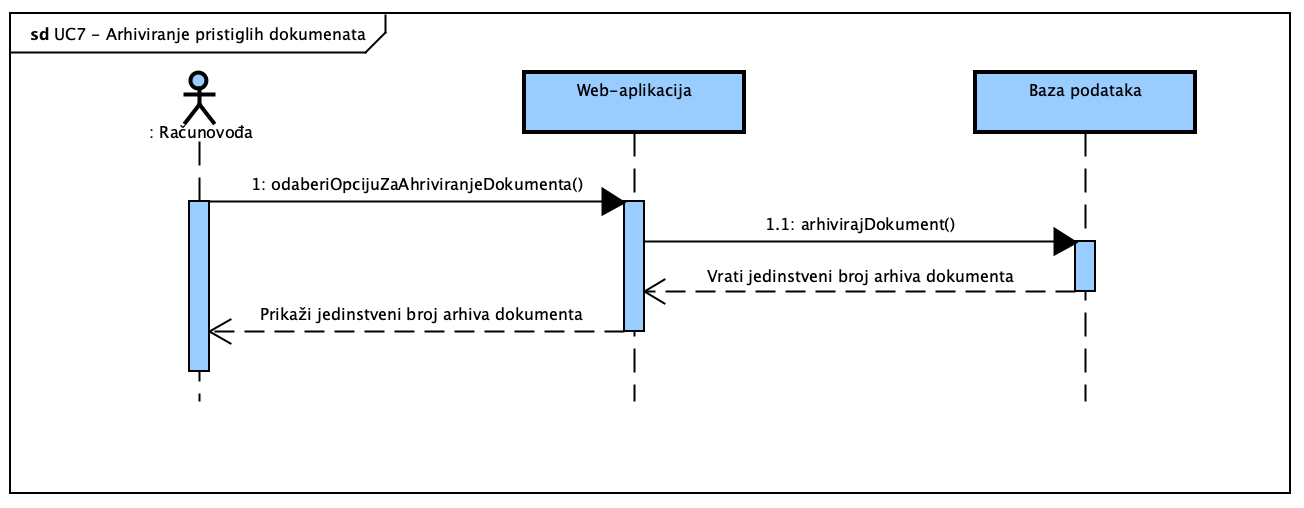
\includegraphics[width=\textwidth]{slike/Sequence_UC07.png}
					\caption{Sekvencijski dijagram za UC07}
					\label{fig:sequence_UC07}
				\end{figure}

				\begin{figure}[H]
					\textbf{Obrazac uporabe UC12 - Registracija novog korisnika}
					\text{Direktor aplikaciji šalje zahtjev za prikaz opcija te odabire opciju za registraciju novog korisnika. Aplikacija bazi podataka šalje zahtjev za formu za registraciju novog korisnika te ju dobiva od baze. Aplikacija prikazuje
					formu za registraciju novog korisnika. Direktor unosi podatke o novom korisniku, uključujući njegovu ulogu, a aplikacija provjerava ispravnost unesenih podataka. Ukoliko je direktor unio neispravne podatke o novom korisniku,
					aplikacija obavještava direktora o neuspjeloj registraciji i vraća ga na formu za registraciju novog korisnika. Ako su uneseni podaci ispravni, aplikacija dojavljuje bazi podataka da registrira novog korisnika. Baza podataka
					pohranjuje podatke o novom korisniku te javlja aplikaciji da je korisnik uspješno unesen. Zatim aplikacija direktoru prosljeđuje da je korisnik uspješno registriran.}
					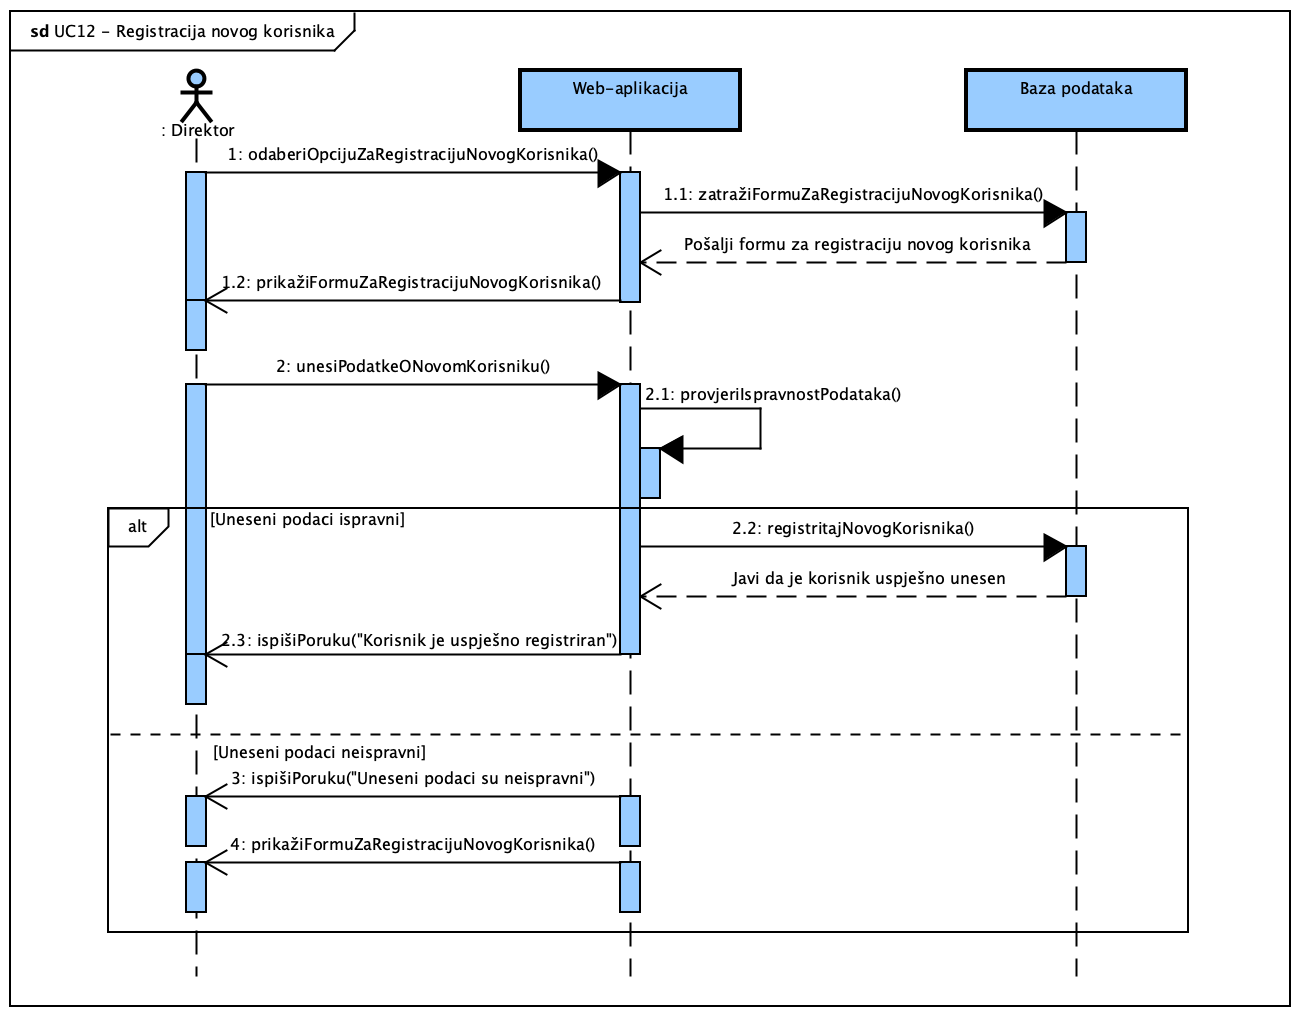
\includegraphics[width=\textwidth]{slike/Sequence_UC12.png}
					\caption{Sekvencijski dijagram za UC12}
					\label{fig:sequence_UC12}
				\end{figure}

				\begin{figure}[H]
					\textbf{Obrazac uporabe UC13 - Brisanje postojećeg korsinika}
					\text{Direktor aplikaciji šalje zahtjev za prikaz opcija te odabire opciju za brisanje postojećeg korisnika. Aplikacija bazi šalje zahtjev za popis svih postojećih korisnika te ga baza vraća aplikaciji koja ga zatim prikazuje direktoru.
					On odabire korisnika kojeg želi obrisati. Aplikacija dojavljuje bazi podataka da obriše korisnika. Baza podataka briše korisnika te aplikaciji javlja da je uspješno obrisan. Aplikacija tada to javlja direktoru.}
					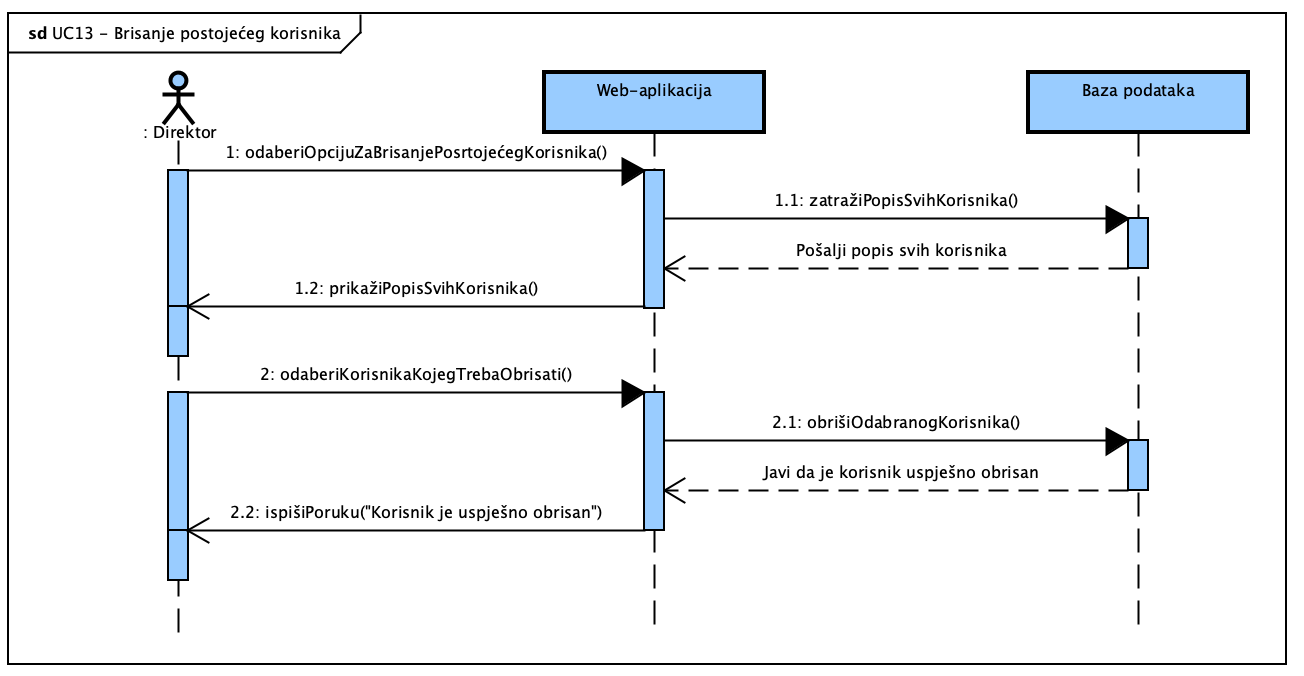
\includegraphics[width=\textwidth]{slike/Sequence_UC13.png}
					\caption{Sekvencijski dijagram za UC13}
					\label{fig:sequence_UC13}
				\end{figure}
			\eject{}
	
		\section{Ostali zahtjevi}
		
			\textbf{\textit{dio 1. revizije}}\\
		 
			\textit{Nefunkcionalni zahtjevi i zahtjevi domene primjene dopunjuju funkcionalne zahtjeve. Oni opisuju \textbf{kako se sustav treba ponašati} i koja \textbf{ograničenja} treba poštivati (performanse, korisničko iskustvo, pouzdanost, standardi kvalitete, sigurnost...). Primjeri takvih zahtjeva u Vašem projektu mogu biti: podržani jezici korisničkog sučelja, vrijeme odziva, najveći mogući podržani broj korisnika, podržane web/mobilne platforme, razina zaštite (protokoli komunikacije, kriptiranje...)... Svaki takav zahtjev potrebno je navesti u jednoj ili dvije rečenice.}
			 
			 
			 
	